\documentclass[a4paper,12pt]{article}
\usepackage[a4paper,top=1.3cm,bottom=2cm,left=1.5cm,right=1.5cm,marginparwidth=0.75cm]{geometry}
\usepackage{cmap}
\usepackage{mathtext}
\usepackage[T2A]{fontenc}
\usepackage[utf8]{inputenc}
\usepackage[english,russian]{babel}
\usepackage{siunitx}

\usepackage{graphicx}

\usepackage{wrapfig}
\usepackage{tabularx}

\usepackage{hyperref}
\usepackage[rgb]{xcolor}
\hypersetup{
colorlinks=true,urlcolor=blue
}
\usepackage{amsmath,amsfonts,amssymb,amsthm,mathtools}
\usepackage{icomma}
\mathtoolsset{showonlyrefs=false}
\usepackage{euscript}
\usepackage{mathrsfs}
\DeclareMathOperator{\sgn}{\mathop{sgn}}
\newcommand*{\hm}[1]{#1\nobreak\discretionary{}
{\hbox{$\mathsurround=0pt #1$}}{}}

%%% Заголовок
\author{Макаров Лев Евгеньевич}
\title{Лабораторная работа №1.4.1

Изучение экспериментальных погрешностей на примере физического маятника
}
\date{\today}

\begin{document}

\begin{titlepage}
	\begin{center}
		{\large МОСКОВСКИЙ ФИЗИКО-ТЕХНИЧЕСКИЙ ИНСТИТУТ (НАЦИОНАЛЬНЫЙ ИССЛЕДОВАТЕЛЬСКИЙ УНИВЕРСИТЕТ)}
	\end{center}
	\begin{center}
		{\large Физтех-школа фотоники, электроники и молекулярной физики}
	\end{center}
	
	
	\vspace{4.5cm}
	{\huge
		\begin{center}
			{\bf Отчёт о выполнении лабораторной работы 1.4.1}\\
			Изучение экспериментальных погрешностей на примере физического маятника
		\end{center}
	}
	\vspace{2cm}
	\begin{flushright}
		{\LARGE Автор:\\ Макаров Лев Евгеньевич \\
			\vspace{0.2cm}
			Б04-306}
	\end{flushright}
	\vspace{8cm}
	\begin{center}
		Долгопрудный 2023
	\end{center}
\end{titlepage}

\section{Введение}

\textbf{Цель работы:} 
\begin{enumerate}
	\item на примере измерения периода свободных колебаний физического маятника познакомиться с систематическими и случайными погрешностями, прямыми и косвенными измерениями
	\item проверить справедливость формулы для периода колебаний физического маятника и определить значение ускорения свободного падения
        \item убедиться в справедливости теоремы Гюйгенса об обратимости точек опоры и центра качания маятника
        \item оценить погрешность прямых и косвенных измерений и конечного результата
\end{enumerate}

\textbf{В работе используются:} 
\begin{itemize}
    \item металлический стержень с опорной призмой
    \item дополнительный груз
    \item закреплённая на стене консоль
    \item подставка с острой гранью для определения цента масс маятника
    \item секундомер
    \item счётчик колебаний электронный
    \item линейки металлические различной длины
    \item штангенциркуль
    \item электронные весы ВЛТЭ-5100
\end{itemize}
\medskip

\section{Теоретические сведения}

Пусть однородный стержень длины $l$ подвешен на оси $O$ на расстоянии $a$ от центра масс $C$. При отклонении стержня от вертикали на малый угол $\varphi$ начинаются колебания стержня, которые можно описать уравнением моментов относительно оси $O$:

\begin{equation}
    I \ddot{\varphi} + m g a \varphi = 0,
\end{equation}

\noindent
где $\varphi$ - угол отклонения маятника от вертикали, $m$ - его масса, $I$ - момент инерции относительно оси подвеса.

\noindent
Получаес уравнение гармонических колебаний, где период равен:

\begin{equation}\label{1form}
    T = 2\pi \sqrt{\frac{I}{mga}}
\end{equation}

\noindent
Используя теорему Гюйгенса-Штейнера получаем:

\begin{equation}
    I = \frac{ml^2}{12} + m a^2
\end{equation}

Подставив это выражение в формулу \eqref{1form}, получим:

\begin{equation}\label{eq3}
    T = 2\pi \sqrt{\frac{\frac{l^2}{12} + a^2}{g a}}
\end{equation}

\noindent

Определим так называемую приведённую длину физического маятника:

\begin{equation}
    l_{\text{пр}} = a + \frac{l^2}{12 a},
\end{equation}

получим, что период равен периоду колебаний математического маятника с длиной $l_{\text{пр}}$.


\begin{figure}[h!]
    \begin{minipage}{0.49\linewidth}
        \center{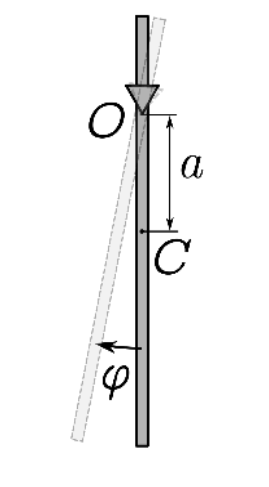
\includegraphics[scale=0.5]{ustan1.png}}
        \caption{\textit{Стержень как физический маятник}}
    \end{minipage}
    \hfill
    \begin{minipage}{0.49\linewidth}
        \center{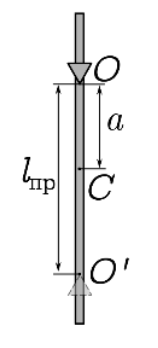
\includegraphics[scale=0.7]{ustan2.png}}
        \caption{\textit{К теореме Гюйгенса}}
    \end{minipage}
\end{figure}

\noindent
В работе также будет изучаться затухание колебаний. Предполагая, что диссипация обусловлена вязким трением, пропорциональным угловой скорости маятника, получим зависимость амплитуды от времени:

\begin{equation}
    A(t) = A_0 e^{-\gamma t}
\end{equation}

\noindent
За время $\tau_{\text{зат}} = 1/\gamma$ амплитуда $A$ колебаний падает в $e$ раз. Отношение времени жизни колебаний к периоду определяет добротность системы:

\begin{equation}\label{calc-Q}
Q = \pi \frac{\tau_{\text{зат}}}{T}
\end{equation}

Наконец, добавим поправки к формуле \eqref{eq3}, учитывающие, конечные массу и размер призмы. Точная формула имеет вид:
\begin{equation}
T = 2\pi \sqrt{\frac{I_{\text{ст}} + I_{\text{пр}}}{m_{\text{ст}} g a - m_{\text{пр}} g a_{\text{пр}}} }
\end{equation}

\noindent
Здесь $I_{\text{пр}}, m_{\text{пр}}, a_{\text{пр}}$ - соответственно момент инерции призмы относительно оси подвеса, её масса и расстояние от оси подвеса до центра масс призмы (знак "минус" в знаменателе означает, что призма находится над осью).

\noindent
Заметим, что $m_{\text{пр}} \sim 10^{-1} \text{ кг}$, $a_{\text{пр}} \sim 1 \text{ см}$, $m_{\text{ст}} \sim 1 \text{ кг} $, $a \geq 10 \text{ см}$, поэтому $I_{\text{пр}}/I{\text{ст}} \sim 10^{-3}$. Это означает, что можно не учитывать $I_{\text{пр}}$. Однако для моментов, создаваемых силами тяжести призмы и стержня, имеем:
\[\frac{M_{\text{пр}}}{M_{\text{ст}}} = \frac{m_{\text{пр}} g a_{\text{пр}}}{m_{\text{ст}} g a} \sim 10^{-2},\]
то есть имеем ошибку до $1\%$ . Будем учитывать эту поправку.

\noindent
Чтобы измерить $a_{\text{пр}}$, будем находить расстояние $x_{\text{ц}}$ от центра масс стержня с призмой до точки подвеса и вычислять $a_{\text{пр}}$ по очевидной формуле: 
\begin{equation}
a_{\text{пр}} = \frac{m_{\text{ст}} a - (m_{\text{ст}} + m_{\text{пр}})x_{\text{ц}}}{m_{\text{пр}}}
\end{equation}

\begin{figure}[h!]
    \center{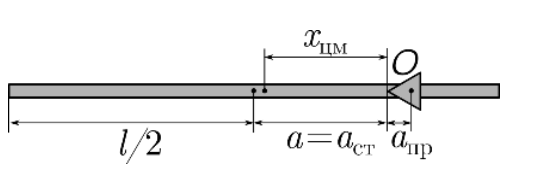
\includegraphics[scale=0.8]{ustan3.png}}
    \caption{.\ \textit{Смещение центра масс из-за подвесной призмы}}
\end{figure}

\noindent
В итоге формула для периода примет вид:
\begin{equation}\label{eq11}
T = 2\pi \sqrt{\frac{\frac{l^2}{12} + a^2}{g (1+\frac{m_{\text{пр}}}{m_{\text{ст}}})x_{\text{ц}}}}
\end{equation}

\section{Оборудование и экспериментальные погрешности}

\textbf{Секундомер:} $\sigma_s = \pm 0,03$ \\ 
\textbf{Линейка металлическая:} $\sigma_\text{лин} = \pm 0,05$ см \\
\textbf{Штангенциркуль:} $\sigma_\text{шт} = \pm 0,005$ см \\
\textbf{Электронные весы ВЛТЭ-5100:} $\sigma_m = \pm 0,1$ г \\

\section{Результаты измерений и обработка данных}
\subsection{Оценка максимальной погрешности}

Оценим, с какой относительной погрешностью $\varepsilon_\text{max}$ имеет смысл измерять период колебаний маятника. Для этого рассчитаем сумарную относительную погрешность измерения приборов (линейки, штангенциркуля и секундомера).\\

Наибольшее расстояние, измеренное штангенциркулем $L^\text{шт}_{max} = 100$ см, а наибольшее измеренное линейкой $L^\text{лин}_{max} = 50$ см. Наибольшие измерения секундомером будут порядка $T = 30$ с. Поэтому относительные погрешности вычисляются так:

\begin{equation}
    \varepsilon_s = 0,10 \%, \text{        } \varepsilon_\text{шт} = 0,01 \%, \text{        }  \varepsilon_\text{лин} = 0,05 \%
\end{equation}

Максимальную относительную погрешность измерения периода колебаний вычислим по формуле:

\begin{equation}
    \varepsilon_\text{max} = \sqrt{ (\varepsilon^s) ^ 2 + (\varepsilon^\text{шт}) ^ 2 + (\varepsilon^\text{лин}) ^ 2} \approx 0,11 \%
\end{equation}

\subsection{Измерение значений параметров установки}

С помощью штангенциркуля измерим длину стердня $l = (98,410 \pm 0,005) \text{ см  } (\varepsilon = 0,01 \%)$. \\

С помощью электронных весов измерим массы стержня $m_\text{0} = (868,3 \pm 0,1 \text{ г}$), призмы $m_\text{пр} = (79,6 \pm 0,1) \text{ г}$ и дополнительного груза $m_\text{г} = (291,0 \pm 0,1) \text{ г}$. Для них соответственно вычислим относительные погрешности:

\begin{equation}
    \varepsilon_\text{0} = 0,01 \%, \text{        } \varepsilon_\text{пр} = 0,13 \%, \text{        }  \varepsilon_\text{г} = 0,03 \%
\end{equation}

\subsection{Определение центра масс стержня}

Снимем со стержня призму и дополнительный груз, после чего с балансируя стержень на подставке с острой гранью определим точку центра масс и определим координату центра масс $x_\text{ц}^\text{ст} = (49,90 \pm 0,13) \text{ см}$. В данном случае погрешность измерения $x_\text{ц}^\text{ст}$ равна ширине подставки.

\subsection{Определение центра масс системы с призмой}

Закрепим призму на стержне, так чтобы нижний конец стержня находился в зоне срабатывания датчика, но не задевал его. Измерим с помощью линейки положение острия призмы на стержне
$x_\text{пр} = (20,00 \pm 0,05) \text{ см}$. Вычислим расстояние от острия призмы до центра масс стержня \\$a = x_\text{ц}^\text{ст} - x_\text{пр} = (29,9 \pm 0,1) \text{ см } (\varepsilon_a = 0,33 \%)$. Погрешность $a$ равна удвоенной погрешности измерений линейки, потому что вычисляется как разность двух величин.\\

Рассчитаем положение центра масс системы стержня с призмой $x_\text{ц}$ по формуле:

\begin{equation}
    x_\text{ц} = \frac{m_0 x_\text{ц}^\text{ст} + m_\text{пр} x_\text{пр}}{m_0 + m_\text{пр}} \approx 47,39 \text{ см}
\end{equation}

Систематическую погрешность измерения $\sigma_{x_\text{ц}}$ можно вычислить по формуле:

\begin{equation}
    \sigma_{x_\text{ц}} = \sqrt{
    \left( \frac{d x_\text{ц}}{d m_0}  \right) ^ 2 \sigma_{m_0} ^ 2 + 
    \left( \frac{d x_\text{ц}}{d x_\text{ц}^\text{ст}}  \right) ^ 2 \sigma_{x_\text{ц}^\text{ст}} ^ 2 + 
    \left( \frac{d x_\text{ц}}{d m_\text{пр}}  \right) ^ 2 \sigma_{m_\text{пр}} ^ 2 + 
    \left( \frac{d x_\text{ц}}{d x_\text{пр}}  \right) ^ 2 \sigma_{x_\text{пр}} ^ 2
    } \approx 0,05 \text{ см}
\end{equation}

Таким образом: $x_\text{ц} = (47,39 \pm 0,05) \text{ см } (\varepsilon_{x_\text{ц}} = 0,10 \%)$.
Так как относительная погрешность измерения $a$ больше $\varepsilon_\text{max}$, то скорректируем $\varepsilon_\text{max}$:

\begin{equation}
    \varepsilon_\text{max} = 0,33 \%
\end{equation}

\subsection{Предварительный опыт по измерению периода колебаний}

Установим маятник на консоли, после чего отклоним его на угол $5^\circ$. Убедившись, что маятник качается без помех, змерим время $n = 20$ колебаний $t = 30,55 \text{ с}$. Вычисли значение $T = \frac{t}{n} = 1,528 \text{ с}$. Теперь по формуле полученной из \eqref{eq3} посчитаем предварительное значение $g$:

\begin{equation}\label{calc-g}
    g = 4\pi^2 \frac{\frac{l^2}{12} + a^2}{a T^2} \approx 9,6 \text{ } \frac{\text{м}}{\text{с}^2}
\end{equation}

Полученное значение отличается от табличного ($9,81 \text{ } \frac{\text{м}}{\text{с}^2}$) на $1,9 \%$.

\subsection{Определение случайной погрешности измерения с помощью секундомера}

Повторим измерения $t$ из предыдущего пункта ещё пять раз, результаты занесём в таблицу:

\begin{table}[!ht]
    \centering
    \begin{tabular}{|l|l|l|l|l|l|}
    \hline
        N (номер измерения) & 1 & 2 & 3 & 4 & 5 \\ \hline
        t, с & 30,54 & 30,55 & 30,56 & 30,56 & 30,56 \\ \hline
    \end{tabular}
\end{table}

Так как результаты измерений отличаются не более чем на приборную погрешность секундомера, то случайная погрешность измерений мала, в сравнении с приборной, и ей иожно пренебречь.

\begin{equation}
    \sigma_t^\text{полн} = \sigma_s = 0,03 \text{ с}
\end{equation}

\subsection{Определение оптимального значения $n$}

погрешность $T$ вычисляется по формуле:

\begin{equation}
    \sigma_T^\text{полн} = \frac{\sigma_t^\text{полн}}{n} = 0,0015 \text{ с}
\end{equation}

Тогда относительная погрешность $\varepsilon_T = 0,10 \% < \varepsilon_\text{max} = 0,11 \%$. Таким образом $n = 20$ является оптимальным значение для проведения измерений.

\subsection{Определение центра масс дополнительного груза}

Для измерения центра масс системы с дополнительным грузом, нужно измерить $x_\text{ц0}$ -- расстояние от центра масс стержня без груза до острия призмы, причем погрешность $\sigma_{x_\text{ц0}}$ равна удвоенной приборной погрешности линейки.

\begin{equation}
    x_\text{ц0} = x_\text{ц} - x_\text{пр} = (27,39 \pm 0,1) \text{ см}
\end{equation}

Закрепим груз в произвольном месте и измерим положение центра масс $x_\text{ц} = (21,50 \pm 0,13) \text{ см}$.

\subsection{Рассчёт положения центра масс груза}

Рассчитаем положение центра масс гуза по формуле:

\begin{equation}
    y = \frac{M x_\text{ц} - m_0 x_\text{ц}}{m_\text{г}} = 2,32 \text{ см}
\end{equation}

$M$ в данном случае -- полная масса маятника. $M = (1238,9 \pm 0,3) \text{ г}$, погрешность равна утроенной приборной погрешности линейки, так как величина получена как сумма трёх величин с погрешностью равной приборной.

\subsection{Измерение периода колебаний маятника по $n$ полным колебаниям}

Проведём измерение периода колебаний по $n$ полным колебаниям для десяти положений груза $y$. Для каждого измерения рассчитаем значение $g$ по формуле \eqref{calc-g}. Результаты запишем в таблицу:

\begin{table}[!ht]
    \centering
    \begin{tabular}{|l|l|l|l|l|l|}
    \hline
        N оп. & $y$, см & $x_\text{ц}$, см & $t$, с & $T$, с & $g,  \text{ м}/\text{с} ^ 2$ \\ \hline
        1 & 2 & 21,43 & 29,97 & 1,499 & 10,0 \\ \hline
        2 & 9 & 23,07 & 29,19 & 1,460 & 10,5 \\ \hline
        3 & 16 & 24,71 & 28,72 & 1,436 & 10,9 \\ \hline
        4 & 23 & 26,36 & 28,58 & 1,429 & 11,0 \\ \hline
        5 & 30 & 28,00 & 28,67 & 1,434 & 10,9 \\ \hline
        6 & 37 & 29,65 & 28,98 & 1,449 & 10,7 \\ \hline
        7 & 44 & 31,29 & 29,44 & 1,472 & 10,4 \\ \hline
        8 & 51 & 32,93 & 30,03 & 1,502 & 10,0 \\ \hline
        9 & 58 & 34,58 & 30,75 & 1,538 & 9,5 \\ \hline
        10 & 65 & 36,22 & 31,54 & 1,577 & 9,0 \\ \hline
    \end{tabular}
\end{table}

\subsection{Определение приведённой длины маятника}

Данный пункт задания не выполнялся во время лабораторной работы.

\subsection{Оценка затухания колебаний маятника}

Для оценки затухания измерим число колебаний $n_\text{зат}$, за которое их амплитуда уменьшилась вдвое: $n_\text{зат} = 267$. $\tau_\text{зат}$ -- время, за которое амплитуда падает в 2 раза, $\tau_\text{зат} = 407,59 \text{ с}$. Добротность $Q$ вычислим по формуле \eqref{calc-Q}:

\begin{equation}
    Q = \pi \frac{\tau_\text{зат}}{T} = 838
\end{equation}

Декремент затухания $\gamma$ вычислим по формуле:

\begin{equation}
    \gamma = - \frac{\ln{0,5}}{\tau_\text{зат}} = 0,0017 \text{ с} ^ {-1}
\end{equation}

\subsection{Оценка погрешности результата вычисления $g$}

Для оценки погрешности измерения $g$ найдём среднее значение $\overline{g} = \frac{\sum{g_i}}{N} = 10,3 \text{ } \frac{\text{м}}{\text{с}^2}$ \\

Случайная погрешность измерения $ \sigma_{g}^\text{случ} = \sqrt{\frac{1}{N  (N-1)}\sum(g_i -\overline{g})^2} \approx 0,2 \text{ } \frac{\text{м}}{\text{с}^2}$ \\

Систематическую погрешность измерения $g$ можно вычислить по формуле:

\begin{equation}
    \sigma_{g}^\text{сист} = \sqrt{
    \left( \frac{d g}{d l}  \right) ^ 2 \sigma_{l} ^ 2 + 
    \left( \frac{d g}{d a}  \right) ^ 2 \sigma_{a} ^ 2 + 
    \left( \frac{d g}{d T}  \right) ^ 2 \sigma_{T} ^ 2
    }
\end{equation}

Для каждого из значений $g$ посчитаем $\sigma_{g}^\text{сист}$ и занесём результаты в таблицу:

\begin{table}[!ht]
    \centering
    \begin{tabular}{|l|l|l|l|l|l|l|l|l|l|}
    \hline
        $g,  \text{ м}/\text{с} ^ 2$,  & 10,0 & 10,5 & 10,9 & 11,0 & 10,9 & 10,7 & 10,4 & 10,0 & 9,5 \\ \hline
        $\sigma_{g}^\text{сист},   \text{ м}/\text{с} ^ 2$ & 0,2 & 0,2 & 0,2 & 0,2 & 0,2 & 0,2 & 0,2 & 0,2 & 0,2 \\ \hline
    \end{tabular}
\end{table}

Получаем, что $\overline{\sigma_{g}^\text{сист}} = 0,2 \text{ } \frac{\text{м}}{\text{с}^2}$ \\

Тогда $\sigma_{g}^\text{полн} = \sqrt{\left( \sigma_{g}^\text{случ} \right) ^ 2 + \left( \overline{\sigma_{g}^\text{сист}} \right) ^ 2} \approx 0,3 \text{ } \frac{\text{м}}{\text{с}^2}$

\subsection{Построение и анализ графика зависимости $T$ от $y$}

График зависимости периода колебаний $T$ от положения груза $y$ представлен на \textit{рис. \ref{graph-1}}. Как видно из графика зависимость имеет минимум. Определим по графику положение минимума $T_{min}^{эксп} = 1,429 \text{ с}$ и сравним его с теоретическим расчетом минимального значения

\begin{equation}\label{T-shit}
    T = 2\pi \sqrt{\frac{J_0 + m_\text{г} y^2}{g M x_\text{ц}}}
\end{equation}


\begin{equation}
            T_{min}^{\text{теор}} = min\left\{2\pi \sqrt{\frac{J_0 + m_\text{г} y^2}{g M x_\text{ц}}}\right\} = 2\pi \sqrt{\frac{J_0}{gMx_{\text{ц}}}} \approx 1,49 \text{ с},
\end{equation}

\subsection{Построение и анализ графика зависимости $T^2x_\text{ц}$ от $y^2$}

Постром график, откладывая по оси абсцисс величину $u = T^2x_\text{ц}$, а по оси ординат величину $v = y^2$. График представлен на \textit{рис. \ref{graph-2}}. как видно из графика точки хорошо ложаться на одну прямую.

\subsection{Применение метода наименьших квадратов}

Методом наименьших квадратов определим параметры $(k,\;b)$  наилучшей прямой $u = kv + b$:

\begin{equation}
    k = \frac{\langle uv\rangle - \langle u \rangle \langle v \rangle}{\langle v^2 \rangle - \langle v \rangle^2} = 0,01 \text{ } \frac{c^2}{\text{см}}
\end{equation}

\begin{equation}
    b = \langle u \rangle - k\langle v \rangle = 48,48\; \text{см}\cdot c^2 
\end{equation}

Найдём их погрешности $(\sigma_k\;и\;\sigma_b)$:

\begin{equation}
    \sigma_k = \frac{1}{\sqrt{10}} \sqrt{\frac{\langle u^2 \rangle - \langle u \rangle^2}{\langle v^2 \rangle - \langle v \rangle^2} - k^2} = 3,9 \cdot 10^{-5}\; \frac{c^2}{\text{см}}
\end{equation}

\begin{equation}
    \sigma_b = \sigma_k\sqrt{\langle v^2 \rangle - \langle v \rangle^2} \approx 0,05\; см \cdot c^2.
\end{equation}

По наклону прямой рассчитаем величину ускорения свободного падения g. Формулу для рассчёта $g$ получим из формулы \eqref{T-shit}:

\begin{equation}
    u = T^2x_\text{ц} = \frac{4\pi^2}{gM} \left( m_\text{г} y^2 + J_0\right) = 
    \frac{4\pi^2m_\text{г}}{gM}y^2 + \frac{4\pi^2J_0}{gM} = kv + b
\end{equation} 

Отсюда следует, что

\begin{equation}
    k = \frac{4\pi^2m_\text{г}}{gM}
\end{equation} 

\begin{equation}
    g = \frac{4\pi^2m_\text{г}}{kM} \approx 9,4 \text{ } \frac{\text{м}}{\text{с}^2}
\end{equation}

\subsection{Оценка погрешности $g$}

Погрешность измерения $g$ в пункте \textit{4.16} вычисляется по формуле:

\begin{equation}
    \sigma_{g} = \sqrt{
    \left( \frac{d g}{d m_\text{г}}  \right) ^ 2 \sigma_{m_\text{г}} ^ 2 + 
    \left( \frac{d g}{d k}  \right) ^ 2 \sigma_{k} ^ 2 + 
    \left( \frac{d g}{d M}  \right) ^ 2 \sigma_{M} ^ 2
    } \approx 0,04 \text{ } \frac{\text{м}}{\text{с}^2}
\end{equation}

\subsection{Сравнение результатов расчёта $g$}

Сравним результат расчёта по пункте \textit{4.16} с непосредственным усреднением, проведённым в пункте \textit{4.13}.\\

Для пункта \textit{4.13}: $g = (10,3 \pm 0,2) \text{ } \frac{\text{м}}{\text{с}^2}$ \\

Для пункта \textit{4.16}: $g = (9,4 \pm 0,04) \text{ } \frac{\text{м}}{\text{с}^2}$ \\

Как видно, расчёт $g$ через МНК гораздо точнее, чем метод из пункта \textit{4.13}, а значит он предпочтительнее.


\section{Обсуждение результатов и выводы}

В ходе работы мы познакомились с систематическими и случайными погрешностями, прямыми и косвенными измерениями. \\

Была подтверждена справедливость формулы для периода колебаний физического маятника. Было посчитано значение ускорения свободного падения двумя различными методами. Были оценены погрешности косвенных измерений и конечного результата.\\

Убедились в справедливости теоремы Гюйгенса об обратимости точек опоры и центра качения маятника.\\

По результатам сделанных измерений можно сделать вывод, что метод наименьших квадратов наиболее подходит для измерения ускорения свободного падения при помощи физического маятника.

\newpage

\begin{figure}[h!]
	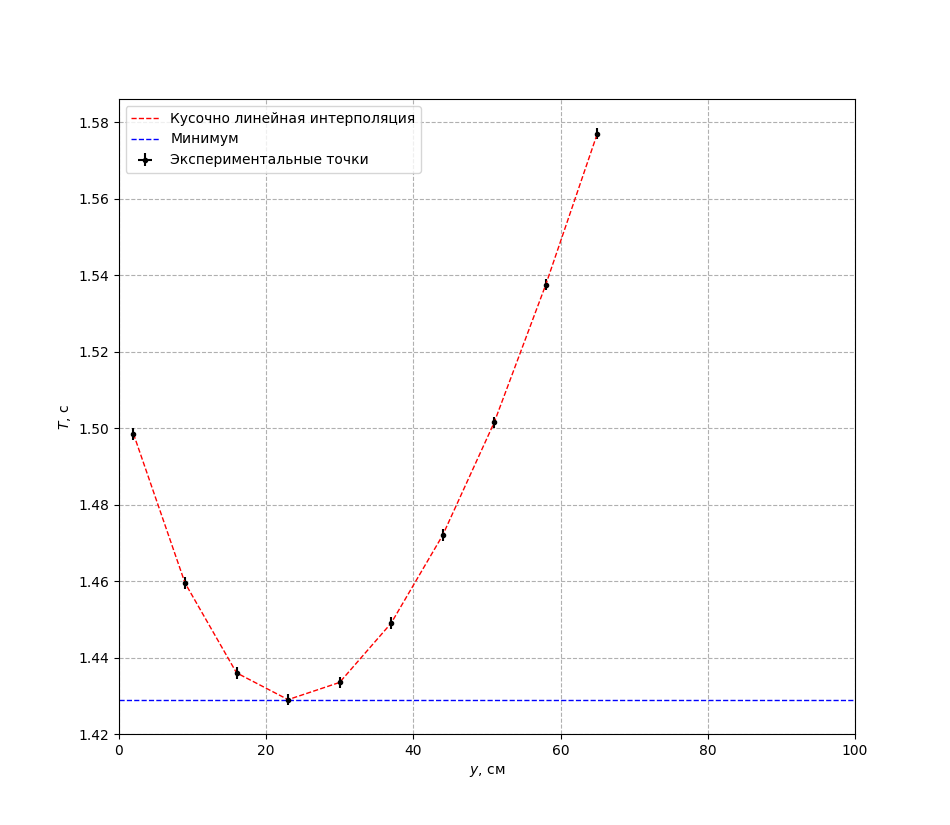
\includegraphics[width=1\linewidth]{graph-1.png}
	\caption{\textit{График зависимости $T$ от $y$.}}
	\label{graph-1}
\end{figure}

\begin{figure}[h!]
    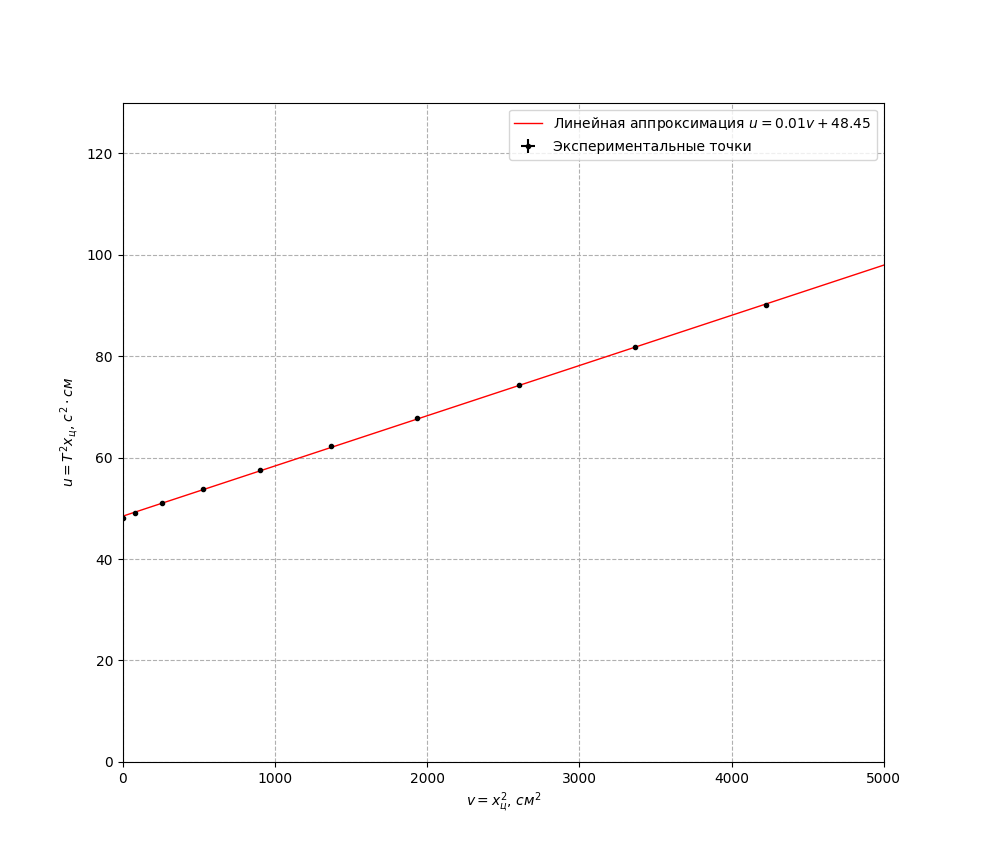
\includegraphics[width=1\textwidth]{graph-2.png}
    \caption{\textit{График зависимости $T^2x_\text{ц}$ от $y^2$.}}
    \label{graph-2}
\end{figure}

\end{document}